\documentclass[../DD0.tex]{subfiles}

\begin{document}

\newcommand{\fetchUML}[4] {

  \begin{figure}[h!]

    \centering
    \hspace*{-#4cm}
    \includegraphics[width=#3\textwidth]{img/UML/#1.jpg}
    \caption{#2}
    \label{fig:#1}

  \end{figure}

}


\def \AccountManager {\texttt{AccountManager}}
\def \DataCollector {\texttt{DataCollector}}
\def \EmergencyDetector {\texttt{EmergencyDetector}}
\def \PaymentGateway {\texttt{PaymentGateway}}
\def \NotificationManager {\texttt{NotificationManager}}
\def \EmergencyDispatcher {\texttt{EmergencyDispatcher}}
\def \FilterManager {\texttt{FilterManager}}
\def \RequestManager {\texttt{RequestManager}}
\def \SetBuilder {\texttt{SetBuilder}}

\section{Architectural Design}
\label{sec:arcdes}

  \subsection{Overview}
  \label{sec:overview}

    The main components of the system are
    \begin{description}
      \item[App] Application installed on users'devices that communicates with the system; its purpose is to show data to the user and forward his/her requests to the Application Server; we will focus on the smartphone app for Andriod or iOS systems, as it is the main front-end application that our clients need
      \item[Application Server] Back-end component on which the logic of the application takes place; it elaborates the requests it receives and interacts with external services and the data layer; we will focus mainly on this component, as it shall handle all the information dispatching from different layers
      \item[Database] Component responsible for data storage; it shall grant ACID properties (Atomicity, Consistency, Isolation and Durability) and shall provide a management service that handles query parallelization and optimization, as data access policies from different accounts
      \item[External Systems] Systems that interact with \texttt{Data4Help} or \texttt{AutomatedSOS}; they handle functionalities not internally developed in the system, such as payment handling and ambulance dispatching
    \end{description}

    \begin{figure}[h!]
      \centering
      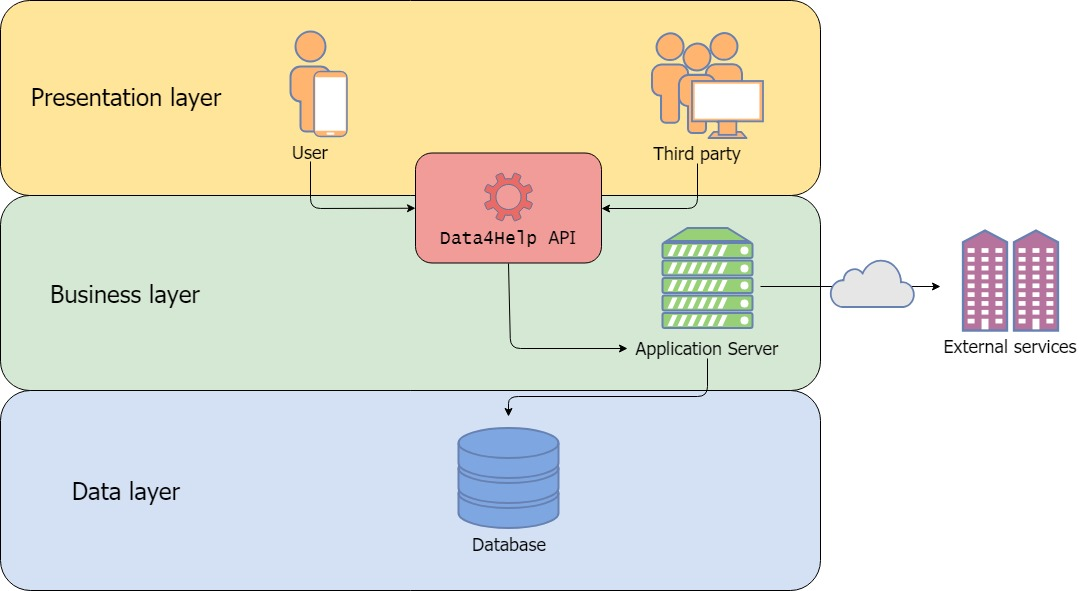
\includegraphics[width=.9\linewidth]{\fetchImg{util/OverallArchitecture.jpg}}
      \caption{Overall architecture of the system}
      \label{fig:overallarchitecture}
    \end{figure}

    The architecture is a three-tier architecture (Figure~\ref{fig:overallarchitecture}): it allows to separate clearly presentation layer, logic layer and data layer. These sets of components will communicate through defined interfaces and will be treated as black boxes during their interaction. This modular approach enhances modifiability and extensibility.


  \subsection{Component view}
  \label{sec:compview}

    In this section we will analyze every high-level component in terms of its subcomponents and provide the main interface interaction between different components. For details on component interfaces see Section~\ref{sec:compinterf}.

      \subsubsection{App}

        The application component is the front-end of the system. Our clients will interact with the system through the front end. We will provide
        \begin{itemize}
          \item A smartphone application, capable of exploiting all of the system functionalities: it shall render data, provide forms for the clients (users and third parties) and communicate with the Application Server
          \item An API that allows more experienced users or other developers to automate communication with our system; the API is particularly useful when third parties need to analyze huge quantities of data that a smartphone graphical interface cannot render
        \end{itemize}

        It is important to note that the smartphone application exploits the API for communication with the Application Server. Every \texttt{Data4Help} or \texttt{AutomatedSOS} service can be required by API communication.

      \subsubsection{Application Server}

        The Application Server holds the application logic. It is the only component of the \textit{business} layer, but it is the most crucial component of the system. Its role is to coordinate the information flow between the user layer and the data layer and to incorporate external systems'services.

        In the architecture the Application Server is the only link to the database. External systems or clients cannot directly access persistent data of our system.

        The Application Server is also the only link to the user interface, as external systems'services cannot directly communicate with users.
%because security issues...?

        Subcomponents of the Application Server are
        \begin{description}
          \item[\AccountManager] This module handles creation, authentication and management of users and third parties'accounts; before exploiting our system's functionalities users and third parties need to be authenticated by this module after providing their credentials
%check whether the data inserted in the registration phase are correct or not
          \item[\DataCollector] This module communicates with users'application and periodically receives data entries, as soon as they're collected by users'wearables
%user and third party application not only user
          \item[\EmergencyDetector] This module is in charge of automatically analyze data entries inserted in the system if their owner subscribed to \texttt{AutomatedSOS}; it is separated from the \DataCollector\ because emergency detection can be exploited in many ways, depending on the medical literature on the topic; this feature should be independant and isolated from the rest of the architecture
          \item[\EmergencyDispatcher] This module builds emergency messages and forwards them tothe SOS system
          \item[\FilterManager] This module composes filter constraints on data entries that can be fetched from the database
          \item[\NotificationManager] This module shall dispatch notifications between user and third party accounts; notifications from users to third parties contain information about user's responses concerning third parties'requests; notifications from third parties to users corcern third parties'single user requests
          \item[\PaymentGateway] This module is in charge of communicating with the external payment system is order to process payments between third parties and TrackMe
          \item[\RequestManager] This module is in charge of composing, verifying and elaborating third parties'requests; it communicates with \FilterManager\ to properly identify which type of data is required and with \NotificationManager\ to keep every client involved in the request updated on its status
%distinguish between single and anonymous group requests(not clear about different info. from/to user to/from third parties
          \item[\SetBuilder] This module generates data-oriented queries for the database, given a particular filter from the \FilterManager; queries can be accepted or declined by the database, depending on the account permissions concerning data entries access
        \end{description}

        % TODO add component diagram

      \subsubsection{Database}

        The database is the only component of the \textit{data} layer. Queries are managed by a DBMS that optimizes and elaborates them in parallel. Data stored in the database is persistent and shall not be lost due to external factors. The database service will not be directly developed by us, but will be bought from the existing ones.

        The \textit{data} layer is only accessible from the Application Server. It won't implement any application logic, except from DBMS functionalities: it will just respond to queries and passively store data.

        An important factor for \texttt{Data4Help} is the data access policy: Data Entries should be available only to the users that produced them, when inserted in the database. If a Data Set is shared to a third party, that third party shall be allowed to retrive Data Entries that belong to that Data Set from the database. Therefore the access policy shall be dinamic and shall consider \texttt{Data4Help} different accounts.

        \begin{figure}[h!]
          \centering
          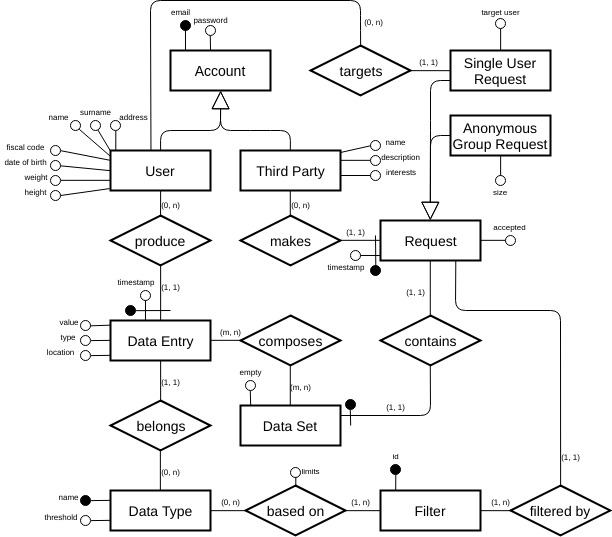
\includegraphics[width=\linewidth]{\fetchImg{util/ER.jpg}}
          \caption{Entity-Relation diagram}
          \label{fig:er}
        \end{figure}

      \subsubsection{External Systems}

        In this section we will present the main external systems that interact with the Application Server.

        \texttt{Data4Help} relies on an external payment handler. The Application Server, once has composed a third party request, evaluates its price and asks third party for payment, by exploiting the external plyment handler service. The service manages the effective payment from the third party to TrackMe and signals errors occurred during the procedure.
%specify that payment gateway also compute the price

        \texttt{AutomatedSOS} relies on an external SOS system. The SOS system dispatches ambulances and handles health emergencies by accepting automated calls. \texttt{AutomatedSOS}, on the Application Server, detects health dangers as soon as they're collected from the front-end components forwards an emergency message to the SOS system.

\clearpage

  \subsection{Deployment view}
  \label{sec:deplview}

\clearpage

  \subsection{Runtime view}
  \label{sec:runtview}
%notes (don't delete)
%orange:user application
%blue:application server
%green:database		DBMS		(interact with appserver only)
%purple:external services		NO :	(interact with appserver only)

\subsubsection{User Account}

\label{sec:userdata}

    \fetchUML
      {run_User_Data}
      {User account}
      {1}           % scale
      {0}           % move left

  \clearpage

%TODO  1)maybe in interaction with DBMS?
% 	     2)description


\subsubsection{Filtering}

\label{sec:filtering}

    \fetchUML
      {run_Filtering}
      {Filtering}
      {1}           % scale
      {0}           % move left

  \clearpage

\subsubsection{AutomatedSOS}

\label{sec:automatedSOS}

    \fetchUML
      {run_AutomatedSOS}
      {AutomatedSOS}
      {1}           % scale
      {0}           % move left

  \clearpage

\subsubsection{Single User request}

\label{sec:singleuser}

    \fetchUML
      {run_Single_Request}
      {Single User request}
      {1}           % scale
      {0}           % move left

  \clearpage

\subsubsection{Anonymous Group request}

\label{sec:anonymousgroup}

    \fetchUML
      {run_Anonymous_Request}
      {Anonymous Group request}
      {1}           % scale
      {0}           % move left

  \clearpage

  \subsection{Component interfaces}
  \label{sec:compinterf}

  \subsection{Selected architectural sytles and patterns}
  \label{sec:stylesandpatterns}

  \subsection{Other design decisions}
  \label{sec:designdecisions}

\end{document}
